\chapter{Úvod do problematiky}

  V této kapitole se seznámíme s pojmy, které jsou pro další postup v práci klíčové. 
  Největší část se zaměří na popsání sportu Ultimate Frisbee, zbytek se věnuje techničtějším pojmům,
  konkrétně aplikačnímu rozhraní, protokolu HTTP a webové službě.

\section{Co je to Ultimate Frisbee}

  Ultimate Frisbee je mladý a dynamicky se rozvíjející sport s létajícím talířem,
  který se hraje od roku 1968~\cite{cald_ultimate}. Hraje jej přibližně sedm miliónů
  hráčů ve více než 80 zemích světa a jeho popularita rok od roku stoupá~\cite{usa_ultimate}.
  Během posledních několika let je běžné sledovat živé přenosy na sportovním kanálu ESPN~\cite{espn}
  z amerických soutěží, především profesionální ligy AUDL~\cite{audl}. Ultimate, jak se mu zkráceně říká, v roce 2015 dokonce získalo
  uznání od Mezinárodního olympijského výboru~\cite{cald_uznani}. Nejčastěji se hraje v kategoriích
  open (muži), ženy, mix (smíšené týmy mužů a žen), junioři (do 19 let) a masters (nad 33 let).

\subsection{Pravidla}

  Popularitě přidává fakt, že jde o celkem vzato nenáročnou hru na vybavení s~jednoduchými pravidly:

\begin{quote}
  \textit{
    Ultimate je kolektivní bezkontaktní sport, v němž vítězí tým, který má na konci hrací doby
    vyšší počet bodů. Hraje se na hřišti o rozměrech cca 100x37 metrů (délka fotbalového hřiště,
    polovina jeho šířky). Na obou koncích hřiště jsou vyznačeny koncové zóny o hloubce cca 18 metrů.
  }
  
  \textit{
    V ultimate proti sobě hrají dva sedmičlenné týmy. Smyslem hry je pomocí přihrávek dopravit disk
    do soupeřovy koncové zóny a jeho chycením v zóně získat bod. Po chycení disku se hráč musí
    zastavit a do 10 vteřin disk přihrát spoluhráči. Povoleným pohybem hráče s diskem je pivotování,
    tedy otáčení se kolem vlastní osy s jednou nohou pevně na zemi. V ultimate hráči často střídají
    útok a obranu při ztrátě disku, ke které dochází záhozem disku do autu, na zem, jeho zachycením
    soupeřem nebo při dlouhém držení disku. Není povolen fyzický kontakt mezi hráči ani přetahování
    o~disk (zdroj:~\cite{cald_ultimate}).
  }
\end{quote}

\begin{figure}[ht!]
  \centering
  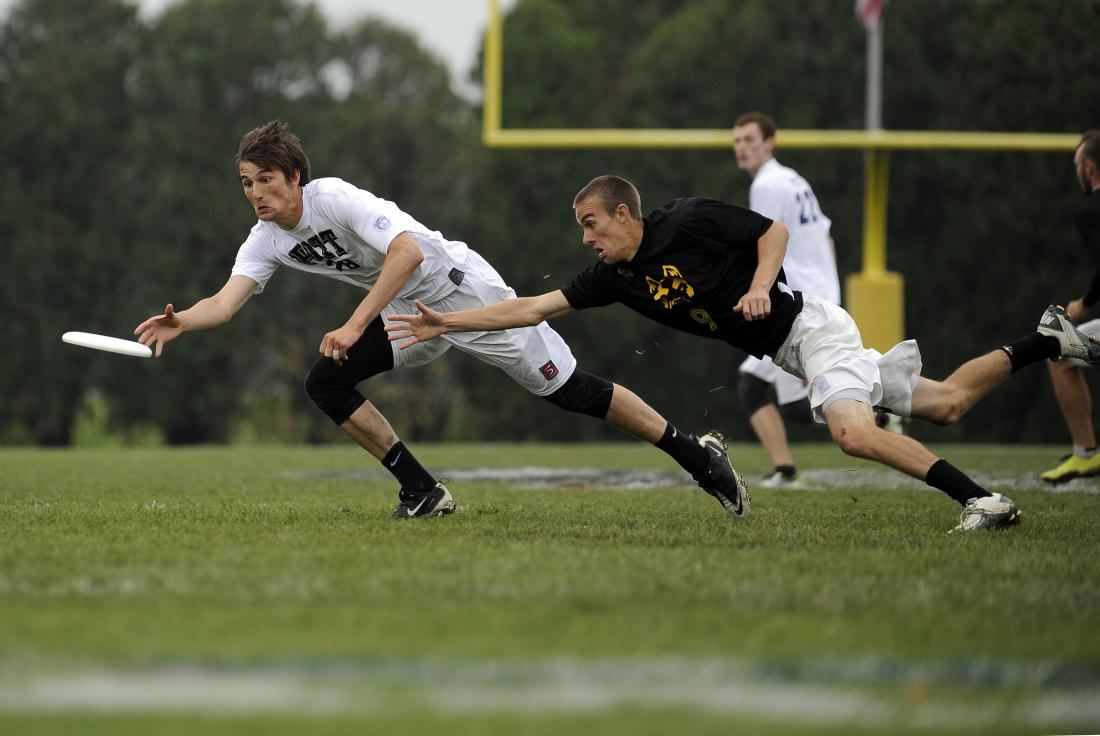
\includegraphics[width=130mm]{./images/ultimate-frisbee.jpg}
  \caption{Fotografie z amerického časopisu TIME ze zápasu mezi
    univerzitními týmy z Pittsburgu a Floridy~\cite{ultimate_time}\label{overflow}
    }
\end{figure}

\subsection{Spirit of the Game}

  Už od počátku je Ultimate Frisbee založeno na hodnotách, jež kladou zodpovědnost za fair play na samotné hráče.
  Očekává se vysoce kompetitivní hra, avšak bez ztráty vzájemné ohleduplnosti a vytracení radosti ze hry.
  Všechna provinění vůči pravidlům řeší samotní hráči. Jako jediná sportovní hra se tak obejde bez rozhodčích, a to i
  na nejvyšších soutěžích, kterými jsou mistrovství Evropy a světa.

  Hraní fair play je otázka cti. Na každém turnaji je vyhlašována cena Spirit of the Game (dále jen \uv{SOTG}),
  která je cenou pro ty, kteří se chovali nejčestněji. Po každém zápase se týmy navzájem ohodnotí
  v podobě číselného hodnocení a cenu pak získá tým s nejvyšším průměrem. Cena SOTG
  je ceněna obdobně jako 1. místo.

\subsection{Ultimate v České republice}

  V České republice zastřešuje sporty s létajícím talířem již od roku 1991~\cite{cald_historie} Česká asociace
  lé\-ta\-jícícho disku (dále jen \uv{ČALD}). V celé republice eviduje desítky zaregistrovaných
  klubů (zvaných taky jako oddílů), které se mezi sebou utkávají v rámci celého roku na akcích zvané turnaje.
  Jenom za loňský rok jich bylo na našem území přes třicet \cite{cald_kalendar}.

  Většina turnajů nebo mistrovství pak trvá zpravidla více dnů, během kterých se odehrají desítky
  utkání. A s přibývajícím počtem hráčů i fanoušků vzniká čím dál větší poptávka po online
  přenosech a statistikách z těchto akcí.

\subsection{Jak vypadá turnaj}

  Běžný turnaj v Ultimate Frisbee se odehrává stylem \textit{skupina-playoff}. Všechny týmy jsou rozlosovány do základních skupin,
  ve~kterých se mezi sebou utkají. Celkový počet vítězství, popř. celkové skóre pak určí pořadí ve skupině a týmy
  jsou nalosovány do vyřazovacích zápasů, tzv. play-off. Vítězné týmy v těchto zápasech postupují turnajem nahoru
  a~poražené bojují o co nejlepší umístění vzhledem k situaci, ve které jsou. Když využijeme analogii z jiných sportů, jde o zápasy typu semifinále,
  kde vítězný tým postoupí do finále a poražený do zápasu o třetí místo. Názornou ukázku turnaje lze vidět na obrázku~\ref{fig:tournament}.

\begin{figure}[ht!]
  \centering
  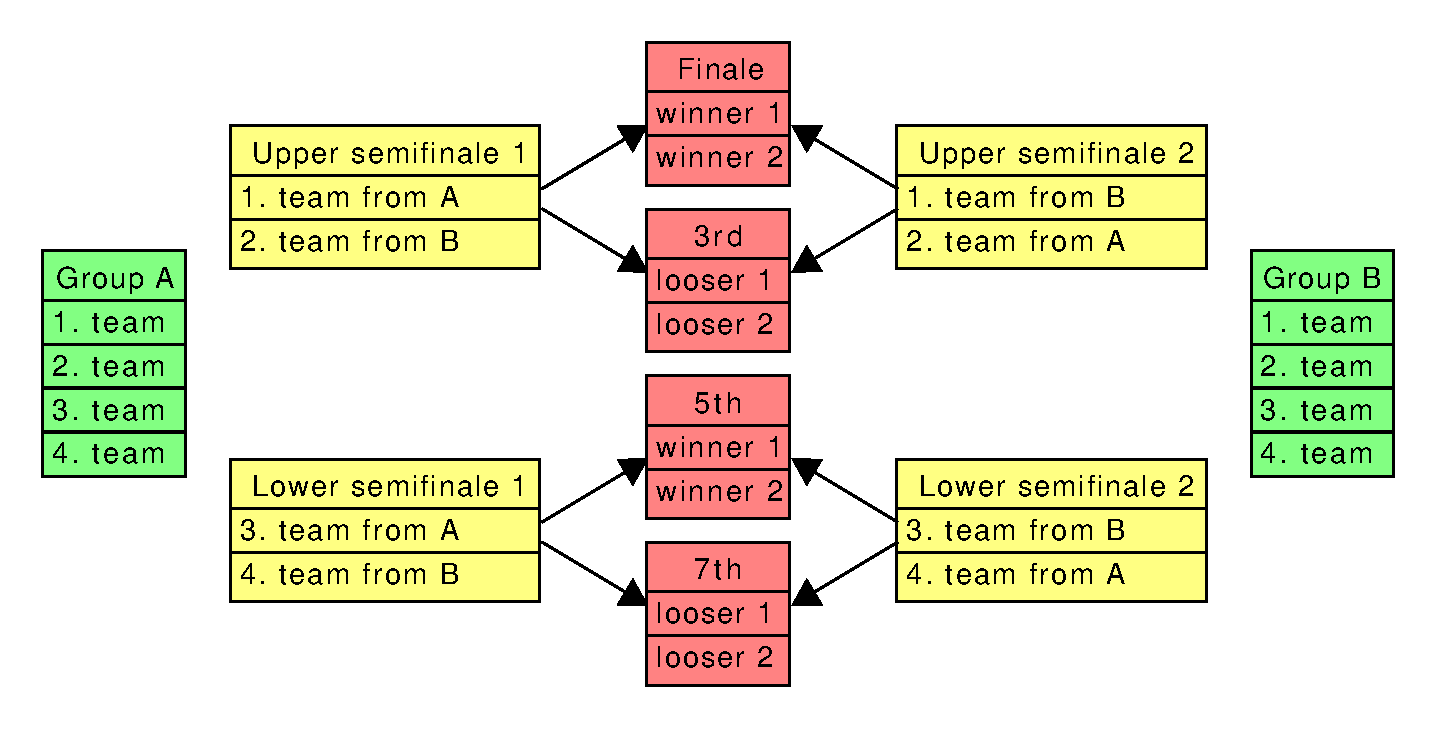
\includegraphics[width=130mm]{./images/turnaj.pdf}
  \caption{Struktura jednoduchého turnaje, kterého se účastní 8 týmů\label{overflow}}
  \label{fig:tournament}
\end{figure}


Dalším typem turnaje, který se běžně hraje, je liga. Týmy jsou pouze v~jedné skupině,
kde je po odehrání všech vzájemných zápasů určeno finální pořadí.

%Několik dní před turnajem se zveřejní rozpis, zpravidla v podobě dokumentu na Google Drive apod.
%Ten je pak během turnajem editovaný a slouží jako jediný zdroj výsledků, který ... 

%Nejdůležitejším údajem jsou výsledky z jednotlivých zápasů. Ty jsou nejčastěji zapisovány
%na papír, který je vystaven na viditelném místě, aby si jej mohlo prohlédnout co nejvíce lidí.

% TODO: Vsechno se doposud pise na papir a je to proste cely na prd.
% TODO: Kdo vsechno turnaj prad, kolik lidi, na turnaji pobyva. Kolik probiha zapasu, treba i paralelne, kdo se o nej stara (navrh ma mobilni app). Co vsechno se da vycist z vysledku.

\section{Aplikační rozhraní}

Častěji se označuje zkratkou API\footnote{Application Programming Interface}.
V informatice se tímto pojmem označuje sbírka procedur, funkcí, tříd
nebo protokolů nějaké knihovny, jež mohou ostatní programátoři používat.
Jde v podstatě o abstrakci, která popisuje rozhraní pro interakci s řadou programových celků,
které programátor využívá namísto toho, aby je sám programoval.
Určuje, jak budou knihovní funkce volány ze zdrojového kódu. API může mít následující vlastnosti.

\begin{itemize}
  % TODO: IDEA: Moznost popsat rozdeleni obecne a konkretni
  \item \textbf{Jazykově závislé API} - Lze volat pouze v daném programovacím jazyce, pomocí základních prvků jazyka.
  \item \textbf{Jazykově nezávislé API} - Jeho použití je možné ve více programovacích jazycích, což je žádoucí vlastnost
    služeb orientovaných na API, které nejsou vázány na určitý systém nebo proces.
    Tato služba pak může být poskytnuta jako webová služba.
\end{itemize}

\section{Protokol HTTP}

% TODO: Zde bych mel uvest zdroj na cizi diplomku.

Protokol HTTP\footnote{Hypertext Transfer Protocol} je základním transportním protokolem na síti internet.
Jde o protokol typu \textit{požadavek-odpověď}. Se serverem naváže klient spojení,
odešle mu požadavek a následně obdrží odpověď. Spojení je pak ukončeno.
Požadavek představuje textový dokument, ve kterém dochází ke specifikování parametru dotazu.
Konkrétní požadavek můžeme vidět na následující ukázce.

\begingroup
\fontsize{9.5pt}{11pt}\selectfont
\begin{verbatim}
GET /api/player/1 HTTP/1.1
Host: catcher.zlutazimnice.cz
\end{verbatim}
\endgroup

Na prvním řádku se nachází název HTTP metody (HTTP obsahuje řadu metod, které mají různý význam, více v tabulce~\ref{tab:http_metody}),
identifikace požadovaného zdroje a verze protokolu. Na následujicích řádcích najdeme tzv.~\uv{hlavičky}
(ve formátu \textit{klíč: hodnota}), které specifikují parametry spojení. Jestliže chceme zaslat společně s požadavkem
nějaká data k dalšímu zpracování, umístí se až za hlavičky a jeden prázdný řádek.

Odpověď serveru je opět textový dokument, ve kterém se nachází verze protokolu a stavový kód,
který reprezentuje výsledek požadavku. Server může vrátit stavový kód z celkem pěti kategorií,
jejich popis je uveden v tabulce~\ref{tab:http_kody}. Za stavovým kódem je ještě krátký textový popisek. Na dalších
řádcích jsou hlavičky a výsledek požadavku, který je oddělen prázdným řádkem, identicky jako v požadavku.
Následující ukázka zobrazuje typickou odpověď z Catchera. 

\begingroup
\fontsize{9.5pt}{11pt}\selectfont
\begin{verbatim}
HTTP/1.1 200 OK
Server: nginx/1.6.3
Date: Mon, 02 May 2016 19:18:18 GMT
Content-Type: application/json; charset=utf-8
Content-Length: 140
Connection: keep-alive
access-control-allow-origin: *
access-control-allow-headers: Content-Type,Authorization,X-Name
access-control-allow-methods: PUT,POST,DELETE,GET

{
  "ranking": null,
  "clubId": 11,
  "firstname": "Pavel",
  "caldId": 976,
  "lastname": "Matoušek",
  "number": 11,
  "nickname": "Maty",
  "id": 1
}
\end{verbatim}
\endgroup
 
 \begin{figure}[ht!]
\centering
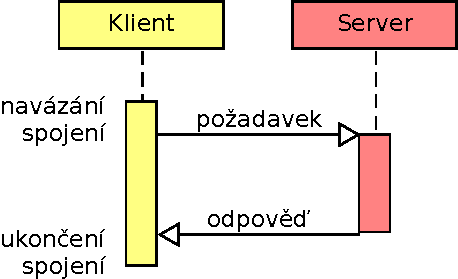
\includegraphics[width=70mm]{./images/http-komunikace.pdf}
\caption{Sekvenční diagram HTTP komunikace; zdroj: autor na základě~\cite{rest_vse}\label{overflow}}
\end{figure}

\begin{table}[ht!]
  \centering
  \begin{tabular}{|l|p{10.1cm}|}
    \hline
    \textbf{Metoda} & \textbf{Význam}\\
    \hline
    GET & Základní metoda, jejíž účel je získat požadovaný zdroj. Neměla by mít žádné postraní efekty, jako tvorba nebo mazaní zdrojů.\\
    \hline
    POST & Metoda pro odesílání dat ke zpracování (data jsou vložena do~těla požadavku). Tato metoda může být použita pro~tvorbu nebo úpravu zdrojů.\\
    \hline
    DELETE & Metoda určená k~mazání zdrojů.\\
    \hline
    PUT & Podobně jako POST slouží k odeslání dat ke zpracování.\\
    \hline
  \end{tabular}
  \caption{Přehled vybraných metod HTTP protokolu v~kontextu této práce~\cite{http_metody}}
  \label{tab:http_metody}
\end{table}

\begin{table}[ht!]
  \centering
  \begin{tabular}{|l|p{9cm}|}
    \hline
    \textbf{Skupina kódů} & \textbf{Význam}\\
    \hline
    1xx & Informační kódy.\\
    \hline
    2xx & Kódy označující úspěšné vykonání požadavku.\\
    \hline
    3xx & Přesměrování - tyto kódy označují odpověď, která obsahuje adresu, na které se nachází požadovaný zdroj.\\
    \hline
    4xx & Chybové kódy označující problém při zpracování, způsobený klientem (odeslání nesprávných dat). Před~opakováním požadavku je nutné opravit vstupní data.\\
    \hline
    5xx & Chybové kódy onzačující problém při zpracování, který vznikl na straně serveru. Požadavek je možné opakovat.\\
    \hline
  \end{tabular}
  \caption{Kategorie návratových kódů HTTP protokolu~\cite{rest_vse}}
  \label{tab:http_kody}
\end{table}

% TODO: uvest zdroj cizi diplomku

\section{Webová služba}

Webová služba je zapouzdřená funkcionalita nějaké aplikace, kterou využívají další aplikace.
Mluvíme tedy o strojové interakci, nevhodné například pro~prohlížení ve webovém prohlížeči.
S veřejně vystavenou webovou službou komunikují ostatní aplikace pomocí definovaného rozhraní.
Pro realizaci API se dnes nejčastěji využívají dva protokoly - SOAP~\cite{soap} a REST~\cite{rest}.
Tyto protokoly jsou přepravené pomocí již zavedených protokolů (hlavně pomocí~HTTP).
